\chapter{Methods}

\label{ch:Methods}

This chapter is organized around three main themes: electromagnetic simulation, physical modeling, and topology optimization, structured as follows:

3.1 introduces the numerical simulation tools;

3.2 provides a complete description of the physical model—its geometric configuration, material parameters, and source settings—presenting both the qualitative framework and the specific numerical values;

3.3 walks through the core modules of the topology optimization process in order, along with their implementation parameters;

3.4 defines the performance metrics used to evaluate the final structure, including the LG mode overlap integral, mode purity, phase winding verification, and optical chirality density analysis.

%===================================================================

\section{Numerical Simulation Methods and Tools}

\subsection{Finite-Difference Time-Domain Method}

To model the electromagnetic behavior, Maxwell's equations are numerically solved using the finite-difference time-domain (FDTD) method, first introduced by Yee in 1966\cite{yee1966numerical}:
\begin{align}
\nabla \times \mathbf{E} = -\frac{\partial \mathbf{B}}{\partial t}, \qquad
\nabla \times \mathbf{H} = \frac{\partial \mathbf{D}}{\partial t} + \mathbf{J}, \qquad
\mathbf{B} = \mu \mathbf{H}, \qquad
\mathbf{D} = \varepsilon \mathbf{E}
\end{align}
It places electric and magnetic field components on staggered spatial grid nodes (Yee cells) and advances them in time using a leapfrog scheme . Numerical stability is governed by the Courant--Friedrichs--Lewy (CFL) condition:
\begin{align}
\Delta t \le \frac{1}{c\sqrt{(1/\Delta x)^2 + (1/\Delta y)^2 + (1/\Delta z)^2}}
\end{align}
where $\Delta t, c$, and $\Delta x, \Delta y, \Delta z$ are the time step, speed of light, and spatial grid sizes, respectively. Perfectly matched layer (PML) absorbing boundary conditions are applied at the computational domain boundaries to mimic open radiation and suppress spurious reflections \cite{berenger1994aperfecctly}.

\subsection{Simulation Environment}

MEEP—an open-source FDTD software package developed at MIT—supports arbitrary non-uniform media distributions, broadband pulse excitation, and parallel computing \cite{Oskooi2009meep}.

Its adjoint optimization extension integrates the forward simulation, adjoint simulation, material interpolation, and projection mapping into a differentiable computational graph. Consequently, the figure-of-merit (FOM) gradients with respect to design variables are efficiently computed via automatic differentiation \cite{Hammond2022high}.

%===================================================================

\section{Physical Model and Numerical Setup}

\subsection{Simulation Geometry}

The simulation domain uses a three-layer vertically stacked structure (see Figure~\ref{fig:sim_geometry_a}): at the bottom is a diamond high-index substrate ($n = 2.40$); in the middle is the monolayer $\text{WS}_2$ excitonic emission layer ($n = 2.40$, thickness set to $1/\text{resolution}$, approximating an atomically thin monolayer); on top is the topology optimization design layer composed of two materials, GaP ($n = 3.31$) and air ($n = 1$), with a design thickness of $t_{\rm design} = 0.257\;\mu\text{m}$ (corresponding to a $2\pi$ phase difference at the excitation wavelength $\lambda = 0.593\;\mu\text{m}$). Surrounded on all sides, top, and bottom by PML boundaries, the computational domain contains a near-field monitor plane positioned directly above the design layer. A circularly polarized point source is embedded in the $\text{WS}_2$ layer; its radiated field travels upward through the design layer, is collected by the near-field monitor, and then propagated to the far-field observation plane via near-to-far-field transformation (N2F).

The lateral dimensions of the computational domain are $S_x = S_y = W_{\rm design} + 2\,d_{\rm pml}$, where the design region side length is $W_{\rm design} = 4.5\;\mu\text{m}$ and the PML layer thickness is $d_{\rm pml} = 0.3\;\mu\text{m}$. The spatial resolution is $50\;\text{grid points}/\mu\text{m}$, giving a discretized design region of $N_x \times N_y = 226 \times 226 \approx 5.1\times10^4$ design degrees of freedom, each node corresponding to an independent density design variable $\rho_j \in [0,1]$. The resulting device footprint is $W_{\rm design}^2 = 20.25\;\mu\text{m}^2$, which is comparable to the scale of reported quantum light source devices \cite{chakravarthi2020inverse}.

GaP at the excitation wavelength $\lambda = 0.593\;\mu\text{m}$ lies below its indirect bandgap ($E_g \approx 2.26\;\text{eV}$), so it can be approximated as a low-loss, high-index dielectric at this wavelength, and it is compatible with electron beam lithography and reactive ion etching fabrication processes.

The target far-field beam waist is set to $w_0 \approx 800\;\text{nm}$ ($\approx 1.35\lambda$). This choice balances two requirements: (i) a compact enough mode footprint so that the intensity ring peak radius $r_\text{peak} = w_0\sqrt{|\ell|/2}$ of the target LG mode remains within the $4.5\;\mu$m design aperture for all six topological charges ($\ell = 0$--$5$), and (ii) a beam waist large enough to produce a well-resolved doughnut profile at the $50\;\text{pts}/\mu$m simulation grid.

\subsection{$\text{WS}_2$ Dipole Source and Valley Selection Rule}

The spontaneous emission from a single exciton in a monolayer $\text{WS}_2$ can be modeled as an electric dipole source. Following the K/K$'$ valley selection rules, the following pair of orthogonal electric dipoles is used to simulate circularly polarized spontaneous emission:
\begin{align}
\mathbf{p} (t) = p_0\!\left[\hat{x}\,e^{-i\omega_0 t} + i\,\hat{y}\,e^{-i\omega_0 t}\right] f (t)
\end{align}
where $f (t)$ is the temporal envelope function, and the $\hat{x}$ and $\hat{y}$ components have equal amplitudes and a $90^{\circ}$ phase difference, together forming a left-circularly polarized (LCP, $\sigma^+$) point source corresponding to the chiral character of K-valley exciton transitions. This is an idealized single circularly polarized equivalent point source and does not account for the actual anisotropic transition dipole moment or multi-valley superposition effects in $\text{WS}_2$ (see Section~\ref{ssec:current_limits} for related limitations).

\subsection{Optical Chirality Density}

\label{ssec:chirality_def}

The optical chirality density is defined following Tang and Cohen (2010) \cite{tang2010optical}:
\begin{align}
C = \frac{\varepsilon_0\,\omega}{2}\,\text{Im}\!\left (\mathbf{E}^{*}\cdot\mathbf{H}\right)
\end{align}
In MEEP's normalized unit system ($\varepsilon_0=\mu_0=c=1$, $\omega = 2\pi f$), this simplifies to:
\begin{align}
C = \pi f\,\text{Im}\!\left (\mathbf{E}^{*}\cdot\mathbf{H}\right)
\end{align}
$C > 0$ indicates RCP dominance; $C < 0$ indicates LCP dominance. To quantify how much the local field enhances chirality relative to an ideal circularly polarized plane wave, an enhancement factor ($g$-factor) is defined:
\begin{align}
g = \frac{|C|}{C_{{\rm CPL,vac}}}
\end{align}
where $C_{{\rm CPL,vac}}$ is the chirality density reference value for a unit-amplitude circularly polarized plane wave in vacuum \cite{hendry2010ultrasensitive}.

%===================================================================

  

  

\section{Topology Optimization}

This section follows the optimization workflow in order: design variable parameterization (3.3.1) $\to$ density filtering and projection (3.3.2) $\to$ near-to-far-field transformation (3.3.3) $\to$ figure of merit (3.3.4) $\to$ adjoint gradient computation (3.3.5) $\to$ MMA update algorithm (3.3.6). Implementation parameters and algorithmic details are presented alongside each step. Figure~\ref{fig:opt_flowchart} provides a visual overview of the complete optimization loop.

\subsection{Design Variables and Material Interpolation}

Topology optimization uses the material density $\rho (\mathbf{x})\in[0,1]$ at each point in the design region as the design variable, and searches for the optimal material distribution in the continuous density space through iterative numerical optimization \cite{bendsøe1988generating, sigmund2013topology}. The key advantage of this framework is that no structural topology needs to be assumed in advance—the geometry in the design space is free to grow, shrink, or change, giving it much higher design freedom than parametric design methods.

The effective dielectric function of the design region is determined by linear material interpolation:
\begin{align}
\varepsilon (\mathbf{x}) = \varepsilon_{A} + \bar{\rho} (\mathbf{x})\,\bigl (\varepsilon_{B} - \varepsilon_{A}\bigr)
\end{align}
where $\varepsilon_A$ (air, $n=1$) and $\varepsilon_B$ (GaP, $n=3.31$) are the dielectric functions of the two design materials, and $\bar{\rho}$ is the physical density after density filtering and projection (see Section 3.3.2).

\subsection{Filtering and Projection}

To avoid checkerboard patterns and respect minimum feature size constraints, the raw design variable $\rho$ is first smoothed by a conic filter \cite{lazarov2011filters}:
\begin{align}
\tilde{\rho} (\mathbf{x}) = \frac{\displaystyle\sum_{i} w (|\mathbf{x}-\mathbf{x}_i|)\,\rho_i}{\displaystyle\sum_{i} w (|\mathbf{x}-\mathbf{x}_i|)}, \qquad w (r) = \max (0,\; R - r)
\end{align}
The filter radius $R$ is back-calculated from the target minimum feature size of $0.05\;\mu\text{m}$ and an erosion threshold $\eta_e = 0.75$, to ensure that the final structural linewidths are achievable by electron beam lithography.

The filtered density $\tilde{\rho}$ is then pushed toward binary values by a hyperbolic tangent projection \cite{wang2011projection}:
\begin{align}
\bar{\rho} (\mathbf{x}) = \frac{\tanh (\beta\eta) + \tanh\!\left (\beta\bigl (\tilde{\rho} (\mathbf{x})-\eta\bigr)\right)}{\tanh (\beta\eta) + \tanh\!\left (\beta (1-\eta)\right)}
\end{align}
where $\eta$ and $\beta$ denote the projection threshold and sharpness parameter, respectively; $\beta \to 0$ corresponds to a grayscale distribution, whereas $\beta \to \infty$ approaches a fully binary state.

$\beta$ schedule: Starting optimization directly with a high $\beta$ value can trap the gradient descent in local minima, so a strategy of gradually increasing $\beta$ is used. $\beta$ starts at $\beta_0 = 4$, increases geometrically by a factor of $\sqrt{2}$ up to 128, and then doubles to $\beta_{\rm max} = 512$. The maximum number of iterations at each stage is set as follows: low-$\beta$ stages ($\beta \le 32$) get 12 iterations, since the smooth gradient landscape converges faster; mid-to-high-$\beta$ stages ($32 < \beta \le 512$) get 30 iterations to ensure the binarized structure converges fully. At each $\beta$ stage, the iteration result with the best FOM (best-so-far snapshot) is used as the starting structure for the next stage.

\subsection{Near-to-Far Field Transformation}

After the near-field monitor plane above the design region records the complete electromagnetic field components, the far-field mode distribution is obtained via near-to-far-field transformation (N2F). The N2F method is based on the electromagnetic equivalence principle \cite{taflove2005computational, balanis2016antenna}: the $\mathbf{E}$ and $\mathbf{H}$ fields on the monitor surface are replaced by equivalent surface electric and magnetic current sources:
\begin{align}
\mathbf{J}_s = \hat{n}\times\mathbf{H}, \qquad \mathbf{M}_s = -\hat{n}\times\mathbf{E}
\end{align}
These equivalent sources are then propagated to any far-field observation point using the free-space dyadic Green's function:
\begin{align}
\mathbf{E}_{ff} (\mathbf{r}_{ff}) = \mathcal{G}\!\left[\mathbf{E}_{near},\, \mathbf{H}_{near}\right]
\end{align}
Inside the optimization loop, a differentiable N2F formulation is introduced so that the adjoint gradient of the FOM can be mapped back through $\mathcal{G}$, enabling accurate gradient computation. During post-processing after optimization, N2F is also used to reconstruct the far-field complex amplitude at multiple propagation distances $z = k\cdot z_R$ ($k \in \{0, 0.1, \dots, 1.0, 2.0, \dots, 10.0\}$, 20 values in total), to verify that the helical beam's phase structure and chirality are stably maintained as the beam propagates.

\subsection{Figure of Merit}

\label{ssec:FOM}

The optimization objective is to make the far-field light approach the target LG mode in the far-field monitor plane ($z = 10\,z_R$, where $z_R = \pi w_0^2/\lambda$ is the Rayleigh length). The key quantities are defined as follows. Given the far-field complex amplitude $\mathbf{E}_{ff} = (E_{ff,x}, E_{ff,y})$ and a power-normalized ($P_{\text{target}}=1$) LCP target mode field $\mathbf{E}_{target}$:
\begin{align}
P_{\text{target}} = \int_A \left( E_{t,x} E_{t,x}^* + E_{t,y} E_{t,y}^* \right) dA = 1
\end{align}
\begin{align}
P_{\text{sim}} = \int_A \left( E_{\text{sim},x} E_{\text{sim},x}^* + E_{\text{sim},y} E_{\text{sim},y}^* \right) dA = \int_A \left( |E_{ff,x}|^2 + |E_{ff,y}|^2 \right) dA
\end{align}
\begin{align}
\text{Overlap} = \int_A \left( E_{ff,x} E_{t,x}^* + E_{ff,y} E_{t,y}^* \right) dA \label{eq:overlap_def}
\end{align}
where $|\text{Overlap}|^2$ measures the absolute coupling power into the target mode, and $\text{Purity} = \dfrac{|\text{Overlap}|^2}{P_{\text{sim}} \cdot P_{\text{target}}}$ measures the mode shape fidelity normalized by total radiated power.

Purity is a dimensionless ratio and is insensitive to the absolute intensity of the electromagnetic field: when the simulated total power $P_{\text{sim}}\to 0$, Purity can still remain high, which would cause the optimizer to converge to a pathological solution---one where the beam shape matches the target, but with near-zero output power. To simultaneously account for mode shape fidelity and energy coupling efficiency, a logarithmically regularized FOM based on the absolute overlap intensity is introduced. This logarithmic form is inspired by the cross-entropy cost function widely used in neural network training: the $\log$ term prevents the optimizer from ignoring the absolute power level, and its gradient signal remains well-conditioned even when Purity approaches 1 or $|\text{Overlap}|^2$ approaches zero, thus avoiding premature convergence to low-power pathological minima:
\begin{align}
\text{FOM} = \log\!\left (\text{Purity}+\epsilon\right) \;+\; \alpha\,\log\!\left (|\text{Overlap}|^2+\epsilon\right)
\end{align}
where $\epsilon = 10^{-30}$ is a numerical stability term, and $\alpha$ is a weight coefficient, controlling how much the optimizer balances mode shape matching against absolute coupling efficiency. Too small an $\alpha$ and the optimizer tends early on to converge to a low-coupling-power local minimum; too large and it sacrifices mode purity for absolute power. A preliminary search selected $\alpha = 0.1$ as a good balance. Since the optimization minimizes the objective, the code returns $-\text{FOM}$.

\subsection{Adjoint Method}

Computing the gradient $\partial \text{FOM}/\partial \rho_j$ by finite difference—perturbing each design variable one at a time—would be proportional in cost to the number of design variables $N \approx 5.1\times10^4$, which is impractical. The adjoint-variable method requires only two electromagnetic simulations (one forward, one adjoint) to obtain gradients with respect to all design variables, with cost independent of $N$ \cite{lalau2013adjoint}:
\begin{align}
\frac{\partial \text{FOM}}{\partial \rho_j} \;\propto\; \text{Re}\!\left[\int_{\Omega_j} \mathbf{E}_{adj} (\mathbf{r}) \cdot \frac{\partial \varepsilon (\mathbf{r})}{\partial \rho_j}\,\mathbf{E}_{fwd} (\mathbf{r})\; dV\right]
\end{align}
where $\mathbf{E}_{fwd}$ is the forward simulation electromagnetic field, $\mathbf{E}_{adj}$ is the adjoint electromagnetic field obtained by injecting the partial derivative of the FOM with respect to the electromagnetic field as a virtual source in reverse, and $\partial\varepsilon/\partial\rho_j$ is determined by the material interpolation relation in equation (3.7).

In the framework with density filtering and projection mapping, the complete gradient of the FOM with respect to the original design variables $\boldsymbol{\rho}$ must be backpropagated layer by layer using the chain rule:
\begin{align}
\frac{\partial \text{FOM}}{\partial \boldsymbol{\rho}} = \frac{\partial \text{FOM}}{\partial \bar\rho}\cdot \frac{\partial \bar\rho}{\partial \tilde\rho}\cdot \frac{\partial \tilde\rho}{\partial \boldsymbol{\rho}}
\end{align}
Using MEEP's adjoint optimization module, the N2F transformation operator, the FOM, and the filtering/projection chain are integrated into a differentiable computational graph, so that gradients are automatically backpropagated to the original design variables $\boldsymbol{\rho}$.

\subsection{MMA Update and Complete Optimization Workflow}

After obtaining the gradients, the design variables are iteratively updated using the Method of Moving Asymptotes (MMA) algorithm \cite{svanberg1987method}. Compared to gradient descent or Adam optimizers, MMA uses a convex separable programming framework: at each iteration, it builds a convex, separable approximate sub-problem based on current gradient information, and constrains the search step size using dynamically adjusted moving asymptotes, balancing convergence stability and computational efficiency. The MMA solver is implemented via the NLopt library, with design variable bounds $0 \le \rho_j \le 1$ \cite{johnson2014nlopt}.

Figure~\ref{fig:opt_flowchart} shows the complete optimization loop, covering all steps from initialization to structural convergence.


%===================================================================

\section{Performance Metrics}

\label{sec:metrics}

With the target beam waist $w_0 \approx 800\;\text{nm}$ and excitation wavelength $\lambda = 0.593\;\mu$m, the Rayleigh length is $z_R = \pi w_0^2/\lambda \approx 3.4\;\mu$m, giving a far-field evaluation height of $10\,z_R \approx 34\;\mu$m. At this propagation distance, evanescent-wave components---confined within a few wavelengths of the nanostructure surface---have fully decayed, leaving a field dominated entirely by propagating plane-wave components; the resulting mode profile is therefore stable and unambiguous, well-suited for rigorous purity and phase-winding evaluation. Note that $34\;\mu$m still lies within the Fresnel near-field zone from a classical antenna perspective; it is therefore referred to as the \textit{effective far field} for the purpose of LG mode evaluation in this work.This section defines the metrics used to evaluate the performance of the optimized structures. All evaluations are based on post-processing forward simulation results of the final binarized structure $\bar{\rho}^*$, and the evaluation plane is set at $z = 10\,z_R$ ($z_R = \pi w_0^2/\lambda$ is the Rayleigh length) by default. 

\subsection{LG Mode Projection and Mode Overlap Integral}

The optimization objective is to make the far-field match a Laguerre--Gaussian (LG) beam with specific mode indices $(\ell, p)$. The full mathematical form of the LG mode complex amplitude $U_{\ell,p} (\rho,\phi,z)$ has been described in Section 2.1.3; here it is directly used to construct the left-circularly polarized (LCP) target field (equation~(3.11)); the power-normalized target field satisfies $P_{\rm target} = 1$ (equation~(3.9)). The mode overlap integral is defined in equation~(\ref{eq:overlap_def}) of Section~\ref{ssec:FOM} and is used directly here.
\subsection{Modal Purity}

The mode purity $P_{\rm target}$ is defined via the overlap integral as given in equation~(3.14) of Section~\ref{ssec:FOM}:

\begin{align}
\text{Purity} = \frac{|\text{Overlap}|^2}{P_{\text{sim}}\cdot P_{\text{target}}}
\end{align}
where $P_{\rm target} = 1$ by power normalization and $P_{\text{sim}}$ is defined in equation~(3.10). Purity is a dimensionless ratio between 0 (complete mismatch) and 1 (perfect match), insensitive to absolute field intensity. The two metrics---Purity and $|\text{Overlap}|^2$---are complementary and must both be reported to fully characterize device performance (see Section~\ref{ssec:purity_overlap} for a detailed analysis of their decoupling behavior at high topological charges).

\subsection{Phase Winding Verification}

Phase winding analysis is the direct method for verifying the topological charge of the far-field helical beam: the LCP electric field phase is sampled along a circular path at the far-field intensity peak radius:
\begin{align}
r_{\rm peak} = w_0\sqrt{|\ell|/2}
\end{align}
After unwrapping, the total azimuthal phase change is calculated; it should ideally equal $\ell \times 2\pi$ ($\ell = 0$ uses a small-radius circle to avoid the central singularity). The phase winding error $|\Delta\ell/\ell|$ serves as a quantitative indicator of topological charge accuracy.

\subsection{Optical Chirality Analysis}

\label{ssec:chirality_analysis}

The optical chirality density (defined in equations (3.4)--(3.6)) is evaluated at two observation planes:

\begin{enumerate}
  \item \textbf{Near-field plane} (just above the design layer, $z = 0^+$): Evaluates how selectively the nanostructure enhances circular polarization in the near field, reflecting the local chiral response of the structure to the K-valley LCP radiation.
  \item \textbf{Far-field plane} ($z = 10\,z_R$): Verifies whether the near-field chiral character is preserved after propagation to the far field, confirming the polarization purity of the propagating field after evanescent wave decay.
\end{enumerate}

In addition, to analyze how chirality evolves along the propagation axis, the chirality density distribution is computed at 20 cross-sections, $z = k\cdot z_R$ ($k = 0.0, 0.1, \dots, 1.0, 2.0, \dots, 10.0$), building a complete picture of the evolution from near field to far field (see Section~\ref{ssec:chirality_prop}).

\begin{figure}[htb]
\centering
    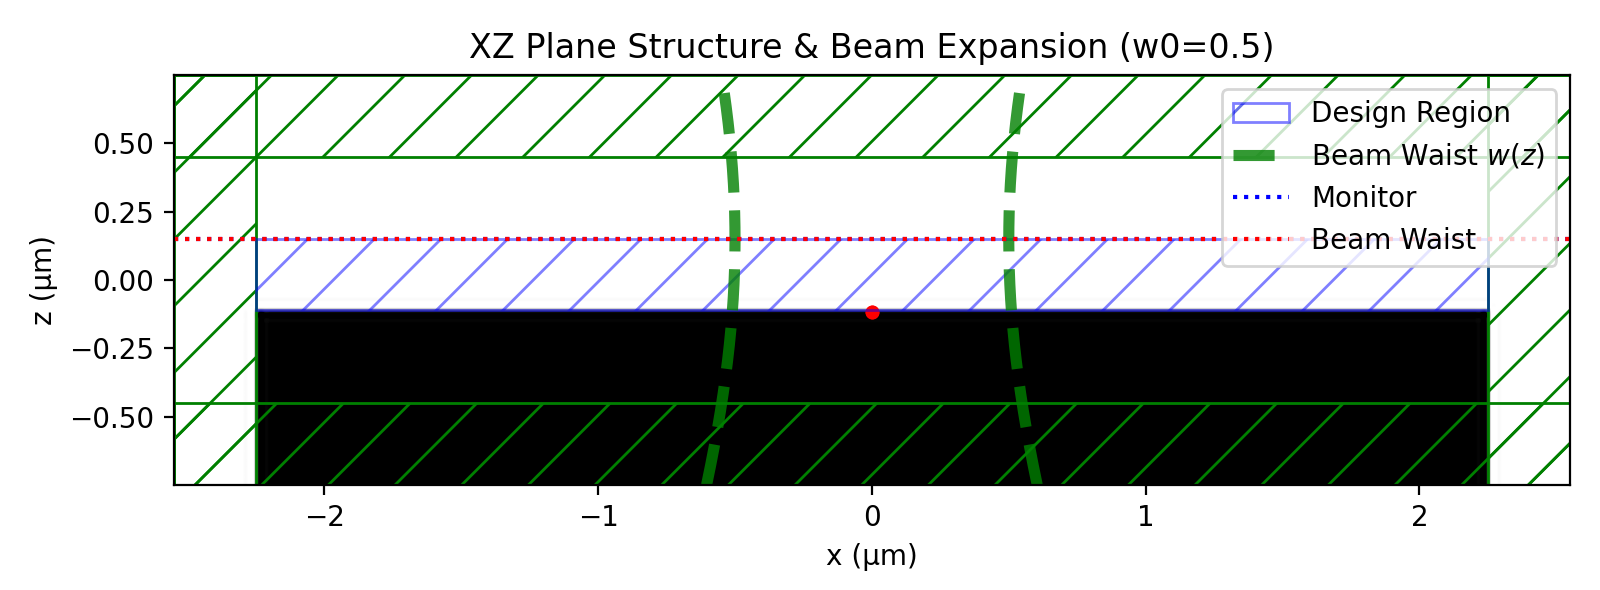
\includegraphics[width=1.0\textwidth]{img/xz_structure_waist.png}
\caption{Cross-sectional diagram of the simulation computational domain. From bottom to top: PML absorbing boundary (bottom), diamond substrate ($n=2.40$), monolayer WS$_2$ excitation layer (with circularly polarized dipole point source), GaP/air topology optimization design layer ($t_{\rm design}=0.257\;\mu$m), near-field monitor plane (red dashed line), air region, and PML (top and sides). The electromagnetic field collected by the near-field monitor is propagated to the far-field observation plane via near-to-far-field transformation (N2F).}
\label{fig:sim_geometry_a}
\end{figure}

\begin{figure}[htb]
\centering
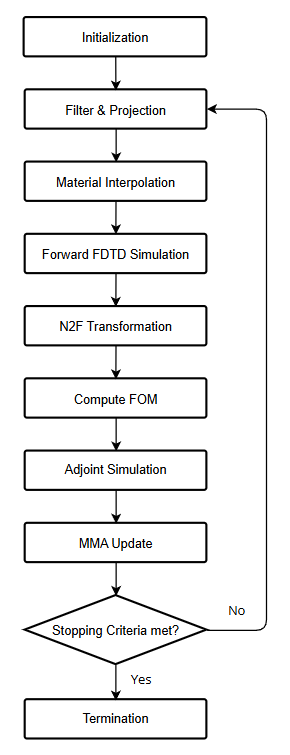
\includegraphics[width=1.0\textwidth,height=18cm,keepaspectratio]{img/workflow.png}
\caption{Topology optimization iteration flowchart. Each iteration performs, in order: forward FDTD simulation, N2F far-field transformation, FOM calculation, adjoint simulation, chain-rule gradient computation, and MMA update. After reaching the iteration limit, if $\beta < \beta_{\rm max}$, $\beta$ is increased and optimization continues (progressive binarization); once $\beta = \beta_{\rm max} = 512$ and convergence is reached, the final binarized structure $\bar{\rho}^*$ is output.}
\label{fig:opt_flowchart}
\end{figure}